\subsection{Распределение вычислительной нагрузки с дроблением блоков сетки}

\subsubsection{Дробление блоков}

Одним из важнейших действий управления расчетной блочно-структурированной сеткой при выполнении вычислений на суперкомпьютере является дробление ее блоков \cite{Rybakov2016WithCut}.
Так как при запуске задач на суперкомпьютере постоянно возрастает степень параллельности (используется все больше параллельных процессов обработки блоков сетки), то для сохранения равномерности распределения блоков по вычислительным процессам требуется уметь измельчать блоки.
Блок сетки может быть разделен на два блока по любому из трех направлениий: $I$, $J$, $K$.

Кроме блоков сетка содержит другие объекты, которые требуют корректировки после разделения блока.
Сюда относятся интерфейсы, описывающие касание блоков друг друга.
На границе расчетной области граничные условия задаются с помощью специальных объектов, которые также должны быть разделены в случае пересечения их линией разреза блока.
Также должны быть по необходимости разделены области, описывающие начальные условия.
Каждыий из этих объектов имеет жесткую привязку к блоку, а значит после дробления может возникнуть
необходимость разделения этого объекта.

Граничные условия и области начальных условий обрабатываются наиболее просто и похожим образом.
Рассмотрим, например, граничные условия в двумерном случае (в координатах $IJ$).

\begin{figure}[ht]
	\centering
	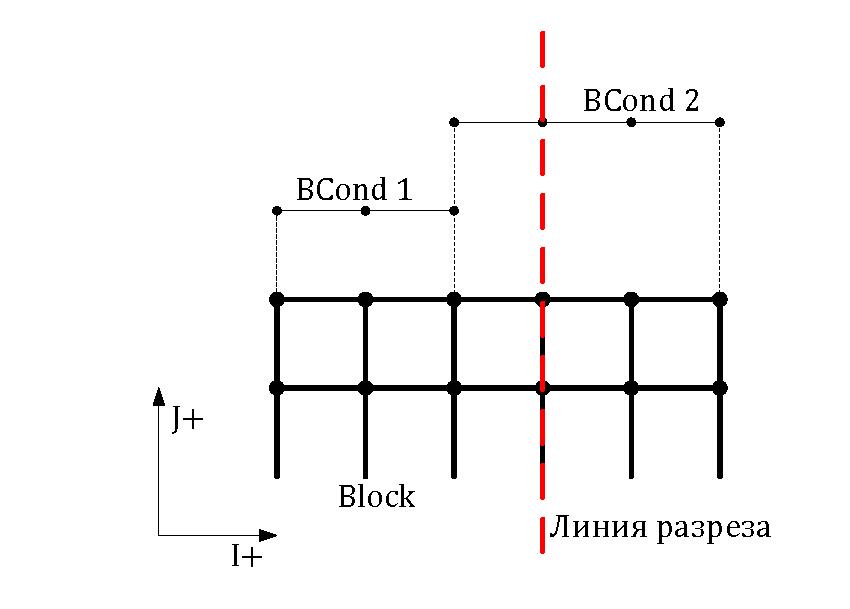
\includegraphics[width=0.6\textwidth]{./pics/text_2_withcut/cut-bcond.pdf}
	\caption{Дробление блока может спровоцировать дробление других объектов сетки.}
	\label{fig:text_2_withcut_cut_bcond}
\end{figure}

Пусть блок Block должен быть разрезан по направлению $I+$ как показано на рис.~\ref{fig:text_2_withcut_cut_bcond}.
Пусть данный блок имеет граничные условия по направлению $J+$.
Тогда возможны два варианта.
Либо линия разреза не пересекает граничное условие, и тогда граничное условие целиком отходит одному из результирующих блоков (BCond 1).
Если же линия разреза проходит через граничное условие, то данное граничное условие также должно быть разделено, и его части отойдут двум результирующим блокам (рис.~\ref{fig:text_2_withcut_cut_bcond2}).

\begin{figure}[ht]
	\centering
	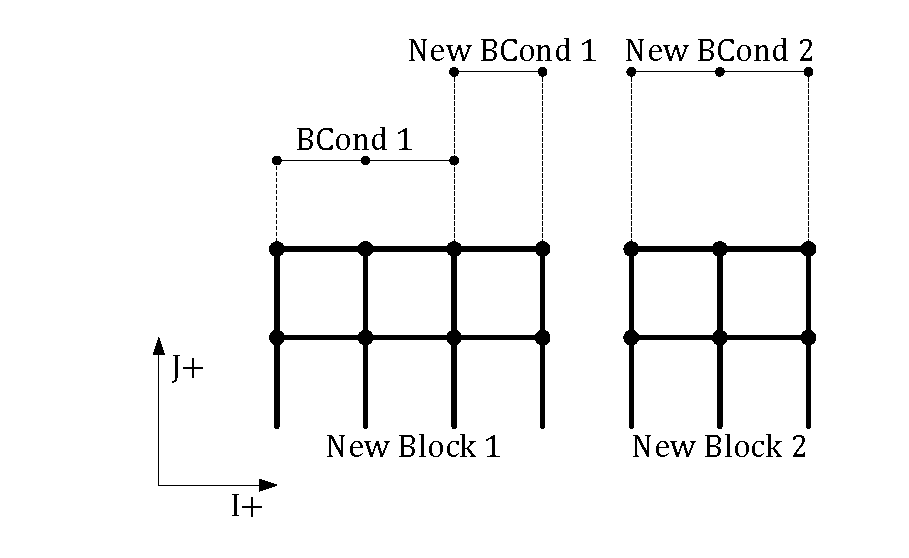
\includegraphics[width=0.6\textwidth]{./pics/text_2_withcut/cut-bcond2.pdf}
	\caption{Разделение граничного условия, спровоцированное дроблением блока.}
	\label{fig:text_2_withcut_cut_bcond2}
\end{figure}

Такая же ситуация может сложиться в отношении областей начальных условий.
В случае дробления интерфейсов могут быть более сложные ситуации дробления.

\subsubsection{Равномерное распределение блоков по вычислительным процессам}

Для равномерного распределения блоков сетки по вычислительным процессам рассмотрим следующую задача разделения множества весов на $m$ различных множеств.

Рассмотрим множество $X$ вещественных чисел $x_i \ge 0$ для $i \in N$, где $N = [1, n]$.
Рассмотрим также множество индексов $j \in M$, где $M = [1, m]$.
Будем говорить, что определено разбиение множества $X$ на $m$ множеств, если введена функция $\gamma(i): N \rightarrow M$.
Множество всех функций разбиения будем обозначать $\Gamma(N, M)$.
Веса результирующих множеств будем определять естественным образом для $j \in M$:
\begin{equation}
	X_j = \sum_{\substack{i \in N \\ \gamma(i) = j}}{x_i}
\end{equation}

Требуется найти такую функцию разбиения $\gamma \in \Gamma(N, M)$, чтобы минимизировать наиболее тяжелое из результирующих множеств: $\min_{\gamma \in \Gamma(N, M)}{\max_{j \in M}{X_j}}$.

Задача может быть расширена на случай распределения вычислительной нагрузки между различными вычислителями суперкомпьютера. При этом формулировка задачи меняется только в части приведения всех узлов к одному показателю с помощью весовых коэффициентов.

Коэффициентом приведения $\kappa(j)$ для $j \in M$ назовем такую положительную функцию $\kappa: M \rightarrow \mathbb{R}_{>0}$, что время выполнения нагрузки $\kappa(j)$ на узле $j$ не зависит от $j$.
Тогда в общем случае задача о равномерном разбиении множества весов на $m$ множеств с коэффициентами приведения $\kappa(j)$ для $j \in M$ формулируется следующим образом.
Требуется найти такую функцию разбиения $\gamma \in \Gamma(N, M)$, чтобы минимизировать наболее тяжелое из результирующих множеств с учетом коэффициентов приведения: $\min_{\gamma \in \Gamma(N, M)}{\max_{j \in M}{\kappa(j) X_j}}$.

Данная задача имеет практическое применение при распределении вычислительной нагрузки между вычислителями гетерогенного суперкомпьютера.

Сформулированная задача является NP-полной, однако ее можно решить приближенно с помощью жадного алгоритма.
В жадном алгоритме будем последовательно обрабатывать все веса, начиная с наибольшего.
Каждый необработанный вес будем относить с наиболее легкому на текущий момент множеству весов.

Приведем без доказательства оценку эффективности работы алгоритма.
Для удобства будем считать, что изначальное множество весов упорядочено по убыванию. 

Определим остаточный член $r_i$ для $i \in N$ по следующей формуле:
\begin{equation}
	r_i = \max{x_i - \frac{1}{m} \sum_{t = i}^{n}{x_t}, 0}
\end{equation}

Тогда можно доказать следующее соотношение
\begin{equation}
	\max_{j \in M}{X_j} - \frac{1}{m} \sum_{j \in M}{X_j} \le \max_{i \in N}{r_i}
\end{equation}

Таким образом, для оценки эффективности описанного жадного алгоритма распределения весов по $m$ множествам достаточно проанализировать ряд остаточных членов, полученный из отсортированного массива распределяемых весов.

Задачу о равномерном распределении весов по результирующим множествам можно применить для равномерного распределения блоков по вычислительным процессам суперкомпьютера в предположении, что все процессы равнозначны (не рассматривается случай гетерогенной системы).
Для этого отметим следующие моменты.
В качестве веса блока нужно взять количество его ячеек.
Так как абсолютно равномерное распределение блоков по вычислительным процессам не всегда возможно, то нужно принять порог максимально допустимого отклонения количества ячеек одного процесса от среднего значения, при достижении которого распределение можно считать успешным.
Экспериментальным путем установлено, что порог максимального отклонения в 10\% является вполне достаточным для достижения эффективного распределения.
Для оценки качества распределения текущего набора весов блоков можно воспользоваться оценками эффективности, приведенными выше.
Если текущее распределение не удовлетворяет допустимому порогу отклонения количества ячеек процесса от среднего значения, то наиболее крупные блоки следует раздробить, после чего повторить оценку распределения.

\subsubsection{Результаты распредедения блоков по процессам}

Предложенные методы равномерного распределения вычислительной нагрузки между узлами суперкомпьютерного кластера были опробованы на суперкомпьютере МВС-10П, находящемся в МСЦ РАН.
Приведем некоторые результаты, которые были получены для двух расчетных сеток.

Первая рассматриваемая сетка, содержит 13 блоков, 80 интерфейсов, 148 граничных условий, 13 областей начальных условий и 5750102 ячейки.
Размер вычислительной окрестности равен 3.

Ниже приведен график, на котором показана статистика общего количества ячеек блоков, а также количества внутренних, граничных и интерфейсных ячеек с учетом кратности.

\begin{figure}[ht]
	\centering
	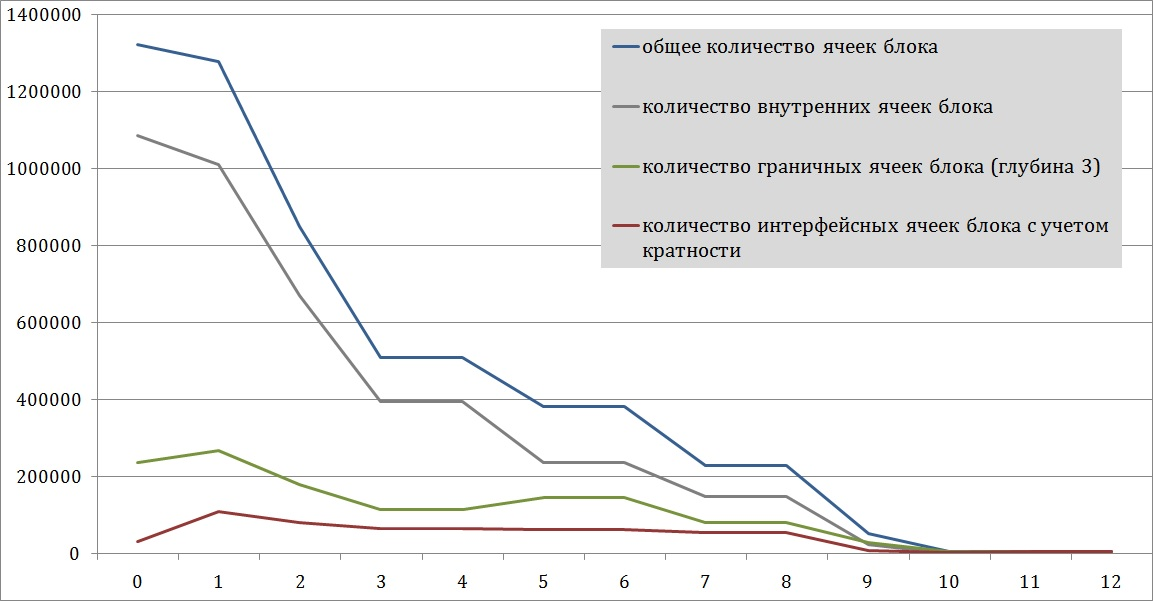
\includegraphics[width=0.6\textwidth]{./pics/text_2_withcut/chart3.jpg}
	\caption{Статистика по количеству ячеек блоков сетки \texttt{vz\_10\_10\_2016}.}
	\label{fig:text_2_withcut_chart3}
\end{figure}

Для этой сетки были проведены вычисления на 128 параллельных процесса.
Приведем статистику распределения блоков по вычислительным процессам для двух различных вариантов: без использования дробления блоков и с использованием дроблений для достижения показателя качества распределения 10\%.

\begin{figure}[ht]
	\centering
	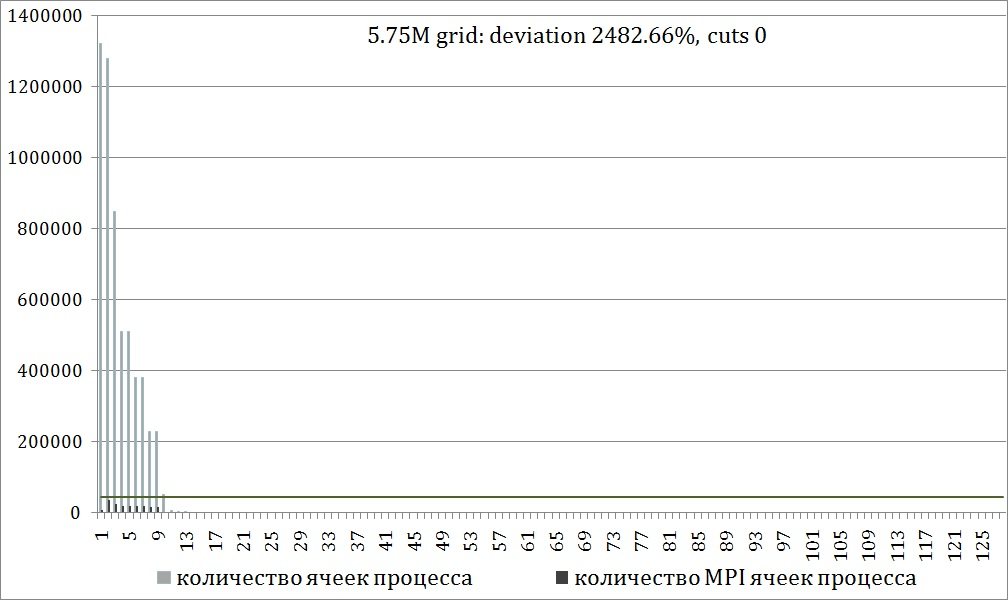
\includegraphics[width=0.6\textwidth]{./pics/text_2_withcut/chart4.jpg}
	\caption{Распределение блоков сетки \texttt{vz\_10\_10\_2016} для 128 процессов без дробления.}
	\label{fig:text_2_withcut_chart4}
\end{figure}

\begin{figure}[ht]
	\centering
	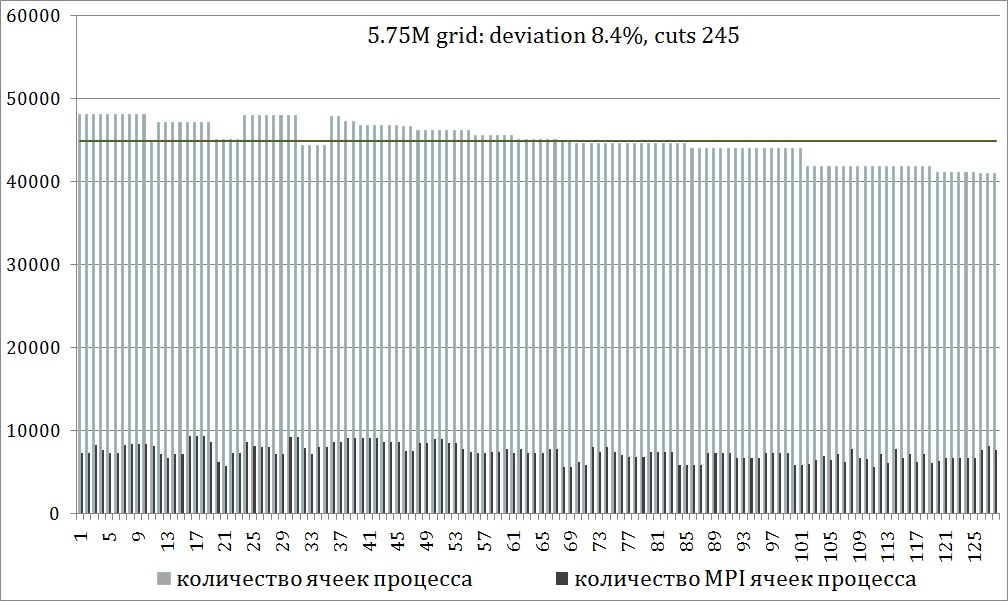
\includegraphics[width=0.6\textwidth]{./pics/text_2_withcut/chart5.jpg}
	\caption{Распределение блоков сетки \texttt{vz\_10\_10\_2016} для 128 процессов с дроблением.}
	\label{fig:text_2_withcut_chart5}
\end{figure}

Аналогичные тестовые запуски производились для сетки, содержащей 300 блоков, 1796 интерфейсов, 1643 граничных условия, 300 областей начальных данных и 94336290 ячейки.
Размер вычислительной окрестности также равен 3.

Ниже приведен график, на котором показана статистика общего количества ячеек блоков, а также количества внутренних, граничных и интерфейсных ячеек с учетом кратности.

\begin{figure}[ht]
	\centering
	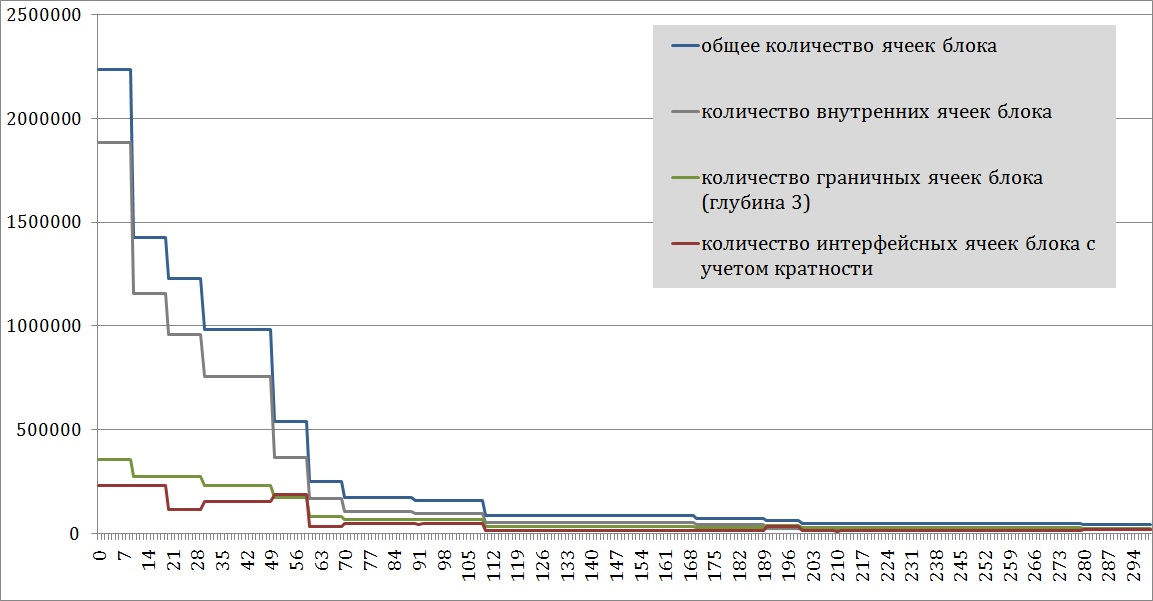
\includegraphics[width=0.6\textwidth]{./pics/text_2_withcut/chart6.jpg}
	\caption{Статистика по количеству ячеек для сетки \texttt{camera\_360\_pill\_nas\_leo\_03\_04}.}
	\label{fig:text_2_withcut_chart6}
\end{figure}

\begin{figure}[ht]
	\centering
	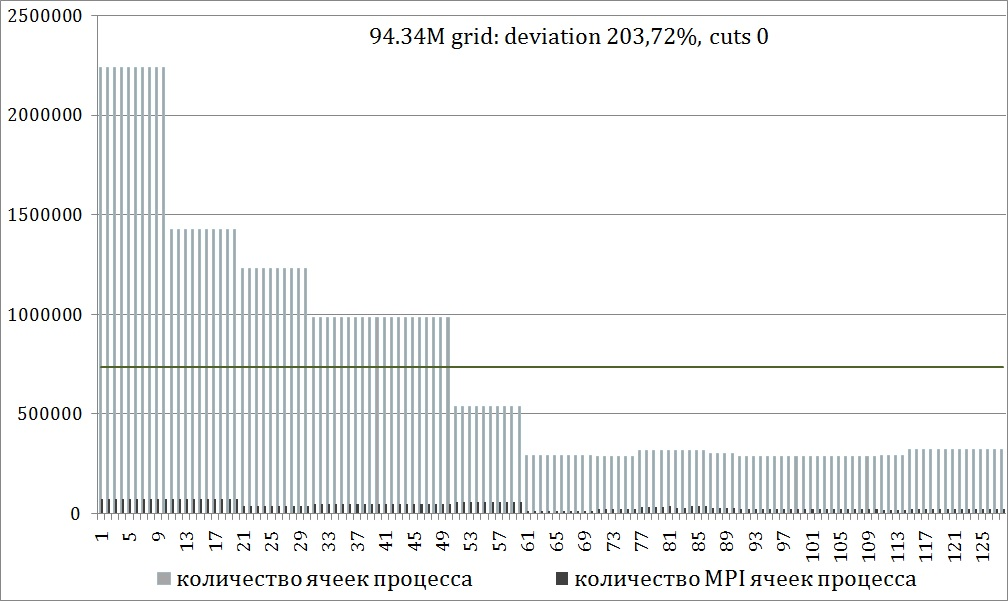
\includegraphics[width=0.6\textwidth]{./pics/text_2_withcut/chart7.jpg}
	\caption{Распределение блоков \texttt{camera\_360\_pill\_nas\_leo\_03\_04}  для 128 проц. без дробления.}
	\label{fig:text_2_withcut_chart7}
\end{figure}

\begin{figure}[ht]
	\centering
	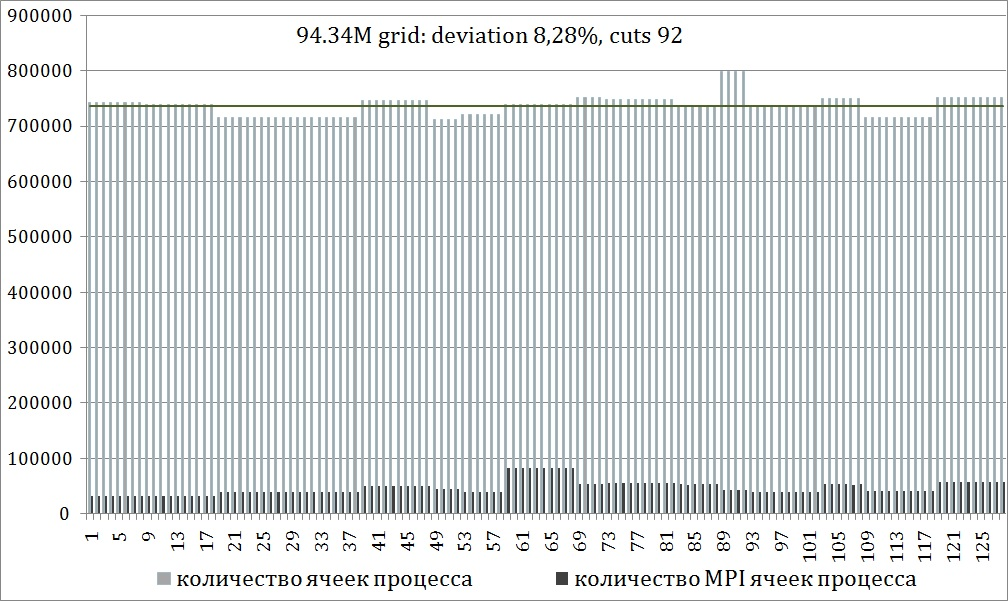
\includegraphics[width=0.6\textwidth]{./pics/text_2_withcut/chart8.jpg}
	\caption{Распределение блоков сетки \texttt{camera\_360\_pill\_nas\_leo\_03\_04} для 128 процессов с дроблением.}
	\label{fig:text_2_withcut_chart8}
\end{figure}

Предложенный механизм равномерного распределения блоков блочно-структурированной сетки между узлами суперкомпьютерного кластера приводит к равномерной загрузке вычислительных ресурсов суперкомпьютерного кластера, что повышает эффективность его использования в расчетах задач газовой динамики. Часто применение такого подхода на большом количестве процессов приводит к кратному ускорению вычислений. Особенно это актуально для сеток содержащих небольшое количество блоков или для сеток, имеющих ярко выраженные крупные блоки.

\subsubsection{Стратегии дробления блоков}

Рассмотрим различные стратегии дробления блоков при недостижении допустимого отклонения при распределении блоков по процессам \cite{Bendersky2017Eff,Bendersky2018Block}.

Применить жадный алгоритм распределения весов блоков по вычислительным узлам.
Если требуемое отклонение наибольшего веса вычислительного узла от среднего значения достигнуто, то завершить работу.
В противном случае разделить максимальный блок пополам по наиболее протяженному направлению, после чего произвести перераспределение.

Такой модифицированный жадный алгоритм с дроблениями пополам будем обозначать UG (от uniform greedy).
Данный алгоритм также всегда завершает работу, однако в отдельных случаях может выполнять необоснованно большое количество дроблений блоков, что приводит к возрастанию количества кросс-ячеек, а значит тормозит межпроцессные обмены между блоками сетки.
Для устранения крупных блоков без лишних дроблений предлагается механизм минимизации количества разрезов блоков.

Прежде всего определим, на какие части может быть разрезан конкретный блок, имеющий размеры $ISize$, $JSize$, $KSize$ и содержащий соответственно $ISize \times JSize \times KSize$ ячеек.

На возможные разрезы блока накладываются следующие ограничения.
Так как блок может быть разрезан только по границам ячеек, то размеры получившихся новых блоков будут кратны одному из значений $ISize \times JSize$, $ISize \times KSize$, или $JSize \times KSize$.
На самом деле целесообразно выполнять разрезы только по наиболее протяженному направлению (пусть это будет $ISize$, для каждого блока это направление будет свое), так как это приводит к минимизации количества кросс-ячеек.
Для сохранения точности расчетов запрещается выполнять разрезы блока слишком близко к границе.
Для этого вводится специальный параметр margin, по которому разрешается деление блока только в сегменте $[margin, ISize - margin]$.
Вводится еще одно ограничение, не позволяющее производить слишком мелкие блоки (задается наименьшее допустимое количество ячеек в результирующем блоке, при котором разрешено дробление).

Алгоритм распределения блоков по вычислительным узлам с минимизацией количества разрезов (в дальнейшем будем обозначать его MCC, от minimal cuts count) будем описывать в следующем виде:

1) Определить среднее ожидаемое количество ячеек, которое должно приходиться на один вычислительный узел, будем обозначать эту величину mid.
Она равна общему количеству ячеек сетки, деленному на количество вычислительных узлов proc.

2) Определить максимально допустимый вес вычислительно узла на текущий момент (будем обозначать через max).
Изначально max берется равным mid.
Однако если в процессе распределения вес какого-либо вычислительного узла превысил mid, то величина max принимает значение веса этого узла.
Таким образом max определяется как максимум из величины mid и весов всех вычислительных узлов.

3) Определить множество всех блоков, которые еще не распределены ни на один вычислительный узел.
Если данное множество пусто, то алгоритм заканчивает работу.

4) Попробовать найти из рассматриваемого множества блоков такой блок, который можно распределить на один из вычислительных узлов так, чтобы вес этого узла не превысил max.
Если таких блоков несколько, то нужно взять такой блок, который максимально приближает вес соответствующего вычислительного узла к отметке max.
Если это удалось, то распределить найденный блок на вычислительный узел и перейти к п. 3.

5) Определить множество допустимых разрезов всех не распределенных на текущий момент блоков.
Каждый потенциальный разрез делит блок на две части.
Определить множество таких потенциальных результирующих блоков и из этих потенциальных блоков выбрать блок веса $w$ и вычислительный узел веса $W$ такие, что $W + w \le max$ и величина $max - (W + w)$ минимальна.
Если такой пары блок-узел не найдено, то найти такую пару, что $W + w > max$ и величина $(W + w) - max$ минимальна.
Такая пара найдется всегда.
После этого выполнить необходимый разрез для получения найденного блока и распределить его на соответствующий вычислительный узел, после чего перейти к п. 2.

Кроме описанных действий данный алгоритм содержит ряд эвристик, не позволяющих проявляться негативным эффектам при возникновении сложных краевых случаев (например, неконтролируемый рост величины max). 
Таким образом, описанный  алгоритм на каждом шаге пытается выполнить такой разрез блока, чтобы максимально приблизить вес некоторого вычислительного узла к ожидаемой в среднем величине загрузки.

Для тестирования и оценки эффективности описанных выше методов распределения блоков блочно-структурированной сетки между узлами суперкомпьютерного кластера использовались три разные сетки, отличающиеся по количеству блоков: test (13 блоков, 5.8 млн. ячеек), train (30 блоков, 10.7 млн. ячеек), ref (136 блоков, 8.5 млн. ячеек).

В качестве целевого вычислительного ресурса брался гомогенный вычислительный кластер, состоящий из 64 узлов.
Величина margin, характеризующая минимальное расстояние разреза от границы блока, бралась равной 5.
На рис.~\ref{fig:text_2_withcut_2_merged_pic} представлены данные применения алгоритмов UG и MCC к каждой из приведенных расчетных сеток. Описание данных на графиках: mid -- средний ожидаемый вес вычислительного узла, dev -- отклонение веса наиболее тяжелого узла от dev, proc -- количество вычислительных узлов, cuts -- количество выполненных разрезов, iface cells и cross cells -- доля интерфейсных и кросс-ячеек среди всех ячеек сетки.

На каждом графике на рис.~\ref{fig:text_2_withcut_2_merged_pic}, представлена гистограмма распределения блоков расчетной сетки по вычислительным узлам.
Каждый столбец гистограммы соответствует одному вычислительному узлу.
Высота столбца – вес соответствующего вычислительного узла.
Если к вычислительному узлу отнесены несколько блоков расчетной сетки, то соответствующий столбец гистограммы разделен на несколько частей, размеры которых отражают веса блоков, также эти части раскрашены в шахматном порядке для повышения наглядности.

\begin{figure}[ht]
	\centering
	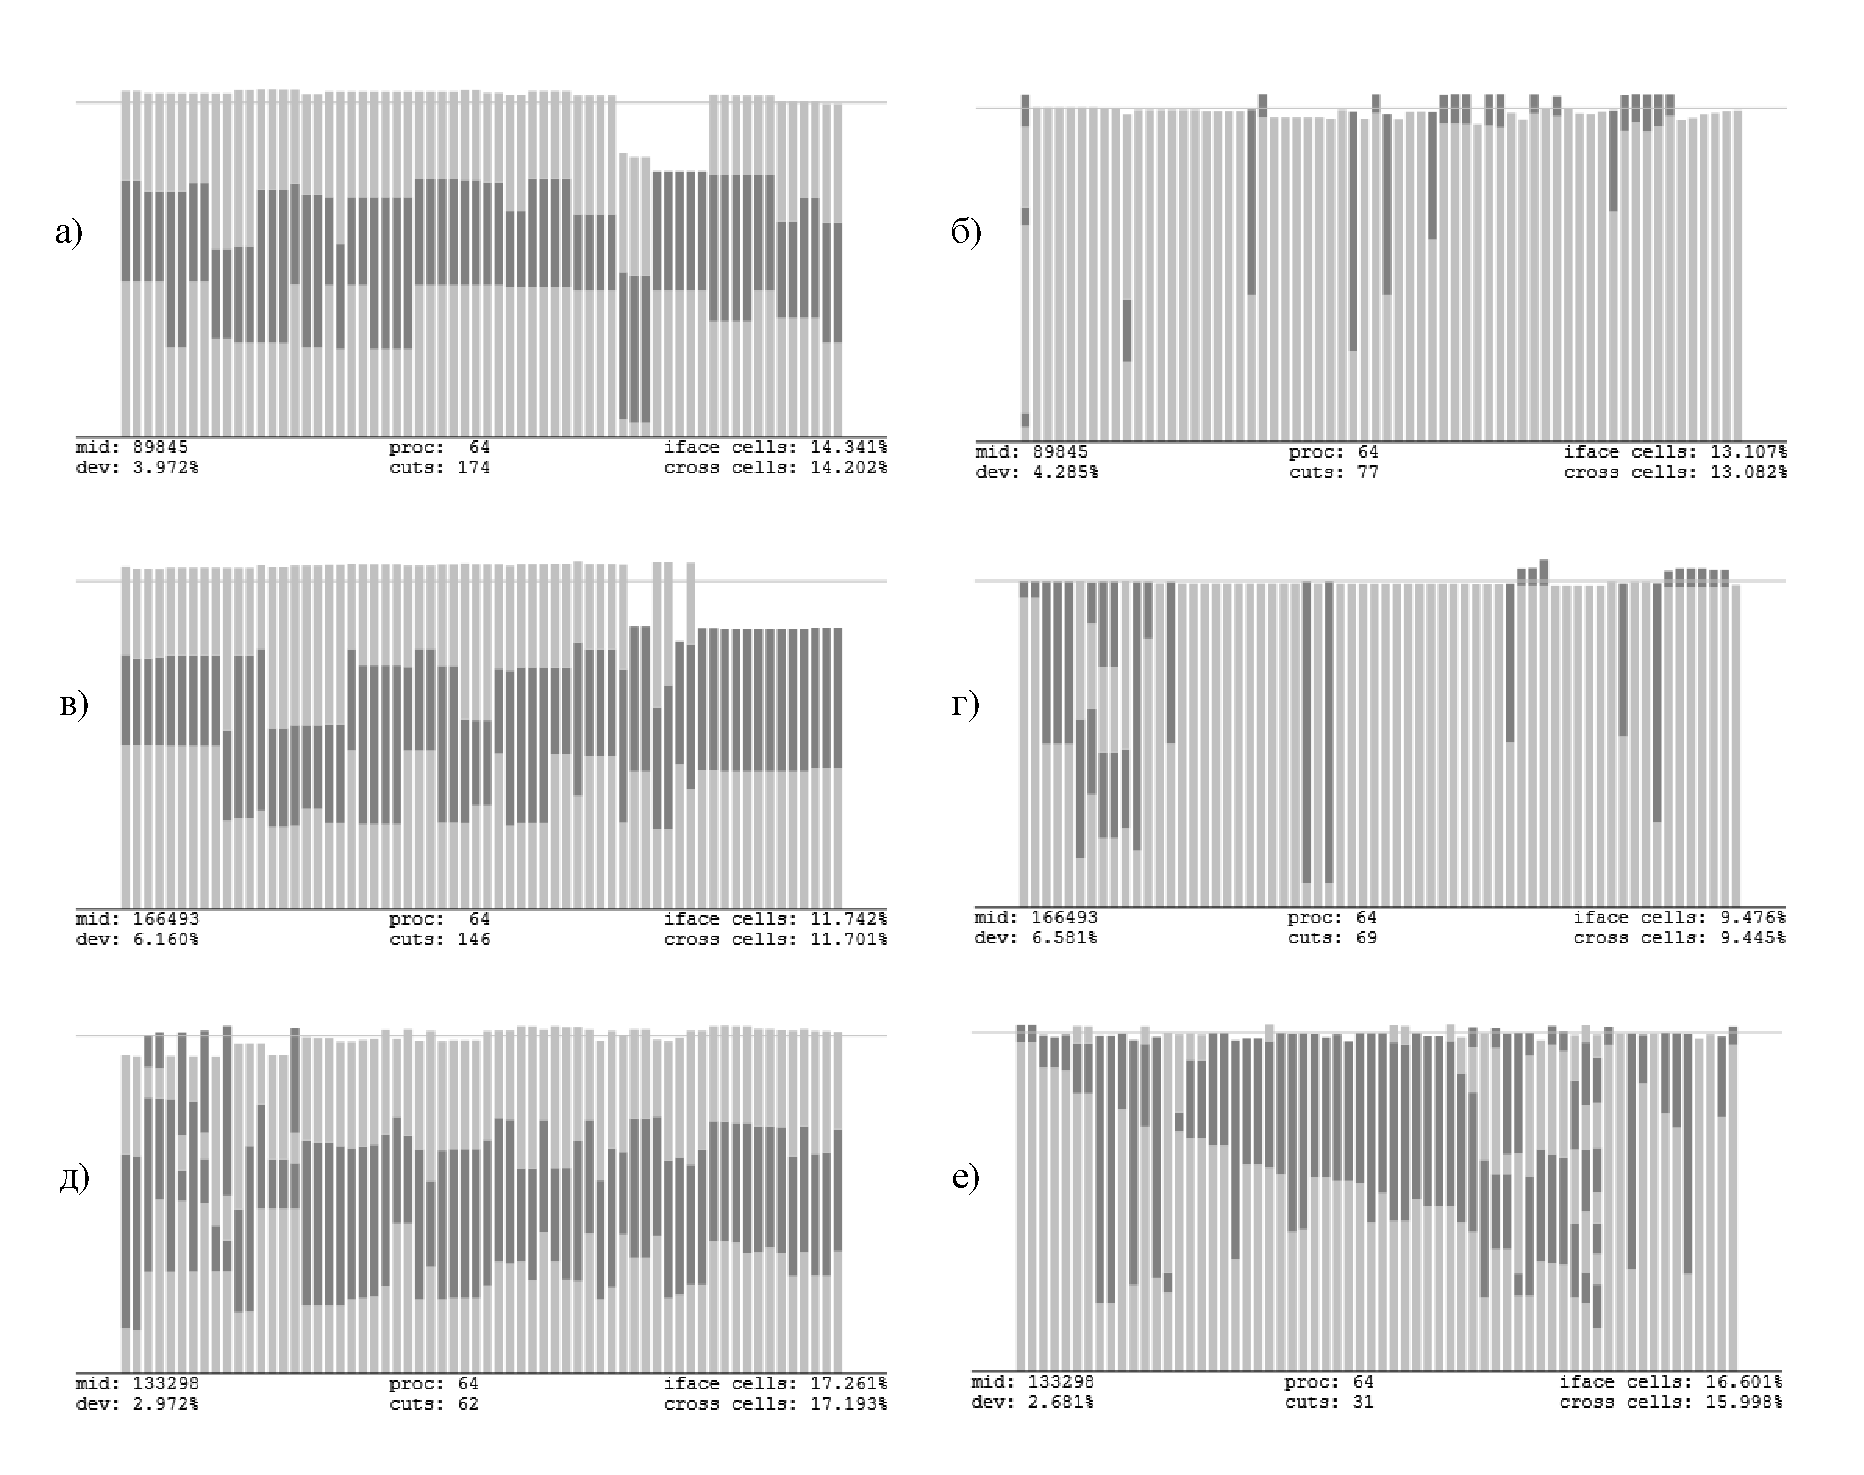
\includegraphics[width=1.0\textwidth]{./pics/text_2_withcut/2-merged-pic.pdf}
	\caption{Гистограммы распределения блоков расчетной сетки по вычислительным узлам суперкомпьютера для сеток            test (а, б), train (в, г), ref (д, е) с помощью алгоритмов UG (а, в, д) и MCC (б, г. е).}
	\label{fig:text_2_withcut_2_merged_pic}
\end{figure}

Результаты сравнения эффективности методов UG и MCC распределения вычислительной нагрузки между узлами суперкомпьютера показывают, что использование метода MCC оправдано, так как с его помощью можно добиться распределения не худшего качества (а зачастую и лучшего), чем при использовании UG.
При этом MCC позволяет существенно сократить количество разрезов блоков сетки для достижения требуемого результата.
Также использование MCC приводит к сокращению количества кросс-ячеек в сетке, что положительно сказывается на скорости межпроцессных обменов данными.
Особенно явно достоинства метода MCC проявляются на сетках с относительно небольшим количеством блоков и наличием ярко выраженных крупных блоков.

Для численного исследования было выбрано модельное плоское двухскачковое ВЗУ высокоскоростного летательного аппарата, описанное в начале статьи.
Для данного объекта проводились численные расчеты на суперкомпьютере с использованием RANS/ILES метода.
Для проведения численных расчетов использовалась блочно-структурированная расчетная сетка, содержащая 172 блока, 848 интерфейсов, 323 граничных условия, 12.8 миллионов ячеек.
Для распределения вычислительной нагрузки для данной сетки использовался алгоритм MCC с дроблением блоков.
В качестве вычислительного поля использовались узлы суперкомпьютера МВС-10П, находящегося в МСЦ РАН, каждый вычислительный узел содержит по 2 микропроцессора Intel Xeon E5-2697v3 (Haswell) [7]. 
Были выполнены запуски расчетов в двух конфигурациях: с запуском двух MPI процессов на каждом процессоре и с запуском четырех MPI процессов на каждом процессоре.
Количество вычислительных узлов варьировалось от 1 до 18.
В качестве эталонного запуска, относительно которого считались ускорения, был выбран запуск на одном узле с двумя MPI процессами на каждом процессоре. 

\begin{figure}[ht]
	\centering
	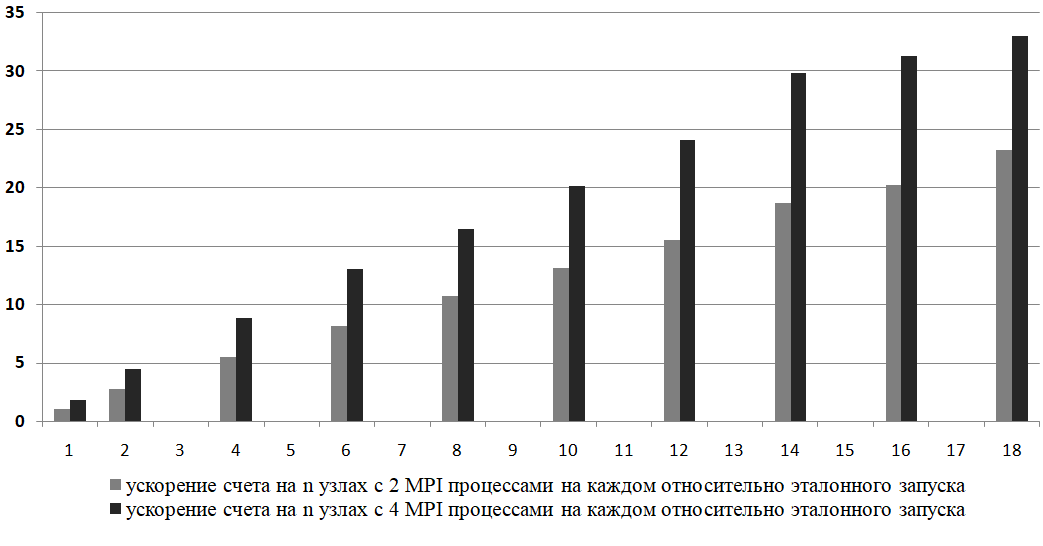
\includegraphics[width=1.0\textwidth]{./pics/text_2_withcut/scaling.png}
	\caption{Ускорение запусков на различном числе узлов относительно эталонного запуска при проведении газодинамических расчетов на модельном входном устройстве воздухозаборника на суперкомпьютере с использованием RANS/ILESметода.}
	\label{fig:text_2_withcut_scaling}
\end{figure}

Из данных, приведенных на рис.~\ref{fig:text_2_withcut_scaling}, можно видеть сверхлинейное ускорение при увеличении количества расчетных узлов.
Так, при использовании 18 узлов с двумя MPI процессами на каждом процессоре было достигнуто 23-хкратное ускорение относительно эталонного запуска.
Такое сверхлинейное ускорение объясняется как равномерностью распределения вычислительной нагрузки между узлами суперкомпьютерного кластера, так и снижением интенсивности и повышением локальности обращений в память при увеличении количества вычислительных узлов.
При использовании 4 MPI процессов на каждом процессоре эффективность счета увеличивается, при этом линейное масштабирование сохраняется.

\subsubsection{Масштабирование вычислений с разными порогами отклонения}

Для анализа эффективности распределения блоков по вычислительным процессам был поставлен эксперимент по выполнению численных  расчетов методом RANS/ILES на блочно-структурированной расчетной сетке, содержащей 94 млн ячеек, а также на отдельном секторе этой сетки с 9,4 млн ячеек \cite{Savin2019RANS}.

Перед вычислениями выполнялась подготовка расчетной сетки для выполнения на 16, 32 и 64 процессах.
При подготовке расчетной сетке использовалось допустимое отклонение 10\%, для подготовки на 64 процессах также использовалось допустимое отклонение в 1\%.

\begin{table}[h!]
\centering
\caption{Характеристики используемых расчетных сеток.}
\bigskip
\label{tbl:text_2_withcut}
\begin{tabular}{ | c | c | c | c | c | }
  \hline
  Описание & Блоки & Интерфейсы & Граничые условия \\ \hline\hline
  360 градусов (94 млн ячеек) & 300 & 1796 & 1643 \\ \hline
  36 градусов (10,7 млн ячеек) & 30 & 152 & 204 \\ \hline\hline
  36 градусов, 16 проц., 10\% откл. & 39 & 224 & 218 \\ \hline
  36 градусов, 32 проц., 10\% откл. & 54 & 340 & 248 \\ \hline
  36 градусов, 64 проц., 10\% откл. & 170 & 982 & 429 \\ \hline\hline
  36 градусов, 64 проц., 1\% откл. & 383 & 2356 & 682 \\ \hline
\end{tabular}
\end{table}

\begin{figure}[ht]
	\centering
	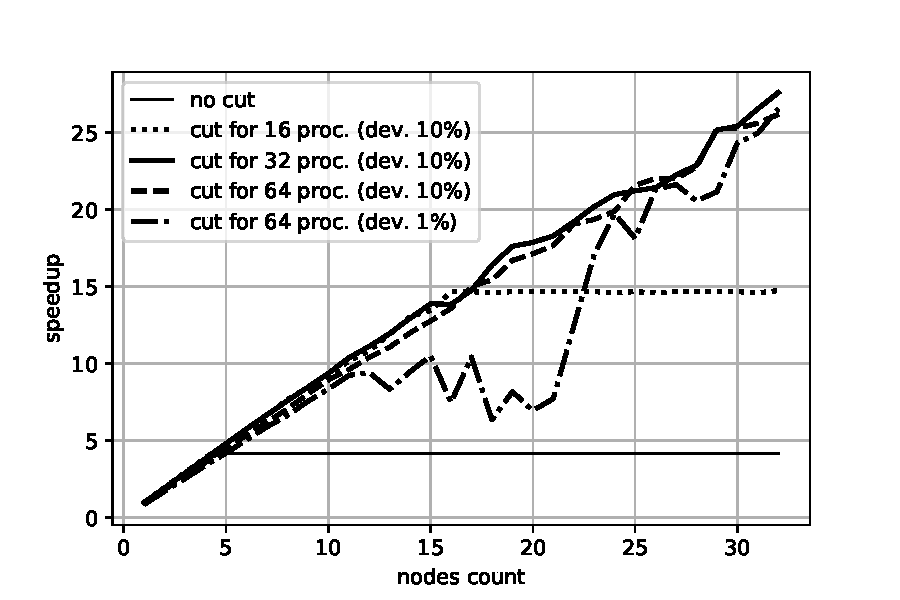
\includegraphics[width=1.0\textwidth]{./pics/text_2_withcut/plot_36_scaling_2.pdf}
	\caption{Масштабирование вычислений при различных параметрах дробления сетки.}
	\label{fig:text_2_withcut_scaling2}
\end{figure}
